\documentclass{mul_poster}

\usepackage{amsmath}
\usepackage{pstricks-add}

\pagestyle{empty}% switch off page numbers on a poster, obviously, and section numbers too.


\usepackage[square,numbers,sort&compress]{natbib}
%% redefinition of the \section command - different spacing + '.' after the section's number
\makeatletter
\renewcommand{\thesection}{\arabic{section}.}
\renewcommand\section{\@startsection{section}{1}{\z@}%
  {-0.1ex \@plus -1ex \@minus -.2ex}%
  {0.2ex \@plus.2ex}%
  {\normalfont\large\bfseries}}%
\renewcommand\subsection{\@startsection{subsection}{1}{\z@}%
  {-0.1ex \@plus -1ex \@minus -.2ex}%
  {0.2ex \@plus.2ex}%
  {\normalfont\bfseries}}%
%% get rid of the ``section'' title in bibliography
\renewenvironment{thebibliography}[1]
     {\@mkboth{\MakeUppercase\bibname}{\MakeUppercase\bibname}%
      \list{\@biblabel{\@arabic\c@enumiv}}%
           {\settowidth\labelwidth{\@biblabel{#1}}%
            \leftmargin\labelwidth
            \advance\leftmargin\labelsep
            \@openbib@code
            \usecounter{enumiv}%
            \let\p@enumiv\@empty
            \renewcommand\theenumiv{\@arabic\c@enumiv}}%
      \sloppy
      \clubpenalty4000
      \@clubpenalty \clubpenalty
      \widowpenalty4000%
      \sfcode`\.\@m}
     {\def\@noitemerr
       {\@latex@warning{Empty `thebibliography' environment}}%
      \endlist}
\makeatother

%% noindentation
\setlength{\parindent}{0pt}
\setlength{\parskip}{1eX}



%% different item symbols
\renewcommand{\labelitemi}{{\color{IMWgreen}$\blacktriangleright$}}
\renewcommand{\labelitemii}{{\color{IMWgreen}$\bullet$}}

% compatibility with revTeX bib style
\makeatletter
\let\href\@secondoftwo
\makeatother

\usepackage[utf8]{inputenc}

\begin{document}

%% \header and footer
\unitlength=1mm
\begin{picture}(100,80)
  \put(-10,-15){
\includegraphics[height=100mm]{graphics/logo_MUL.eps}}                        % MU logo
  \put(70,-30){
\includegraphics[width=680mm,height=120mm]{graphics/IMWbackground.eps}}      % header background
  \put(745,5){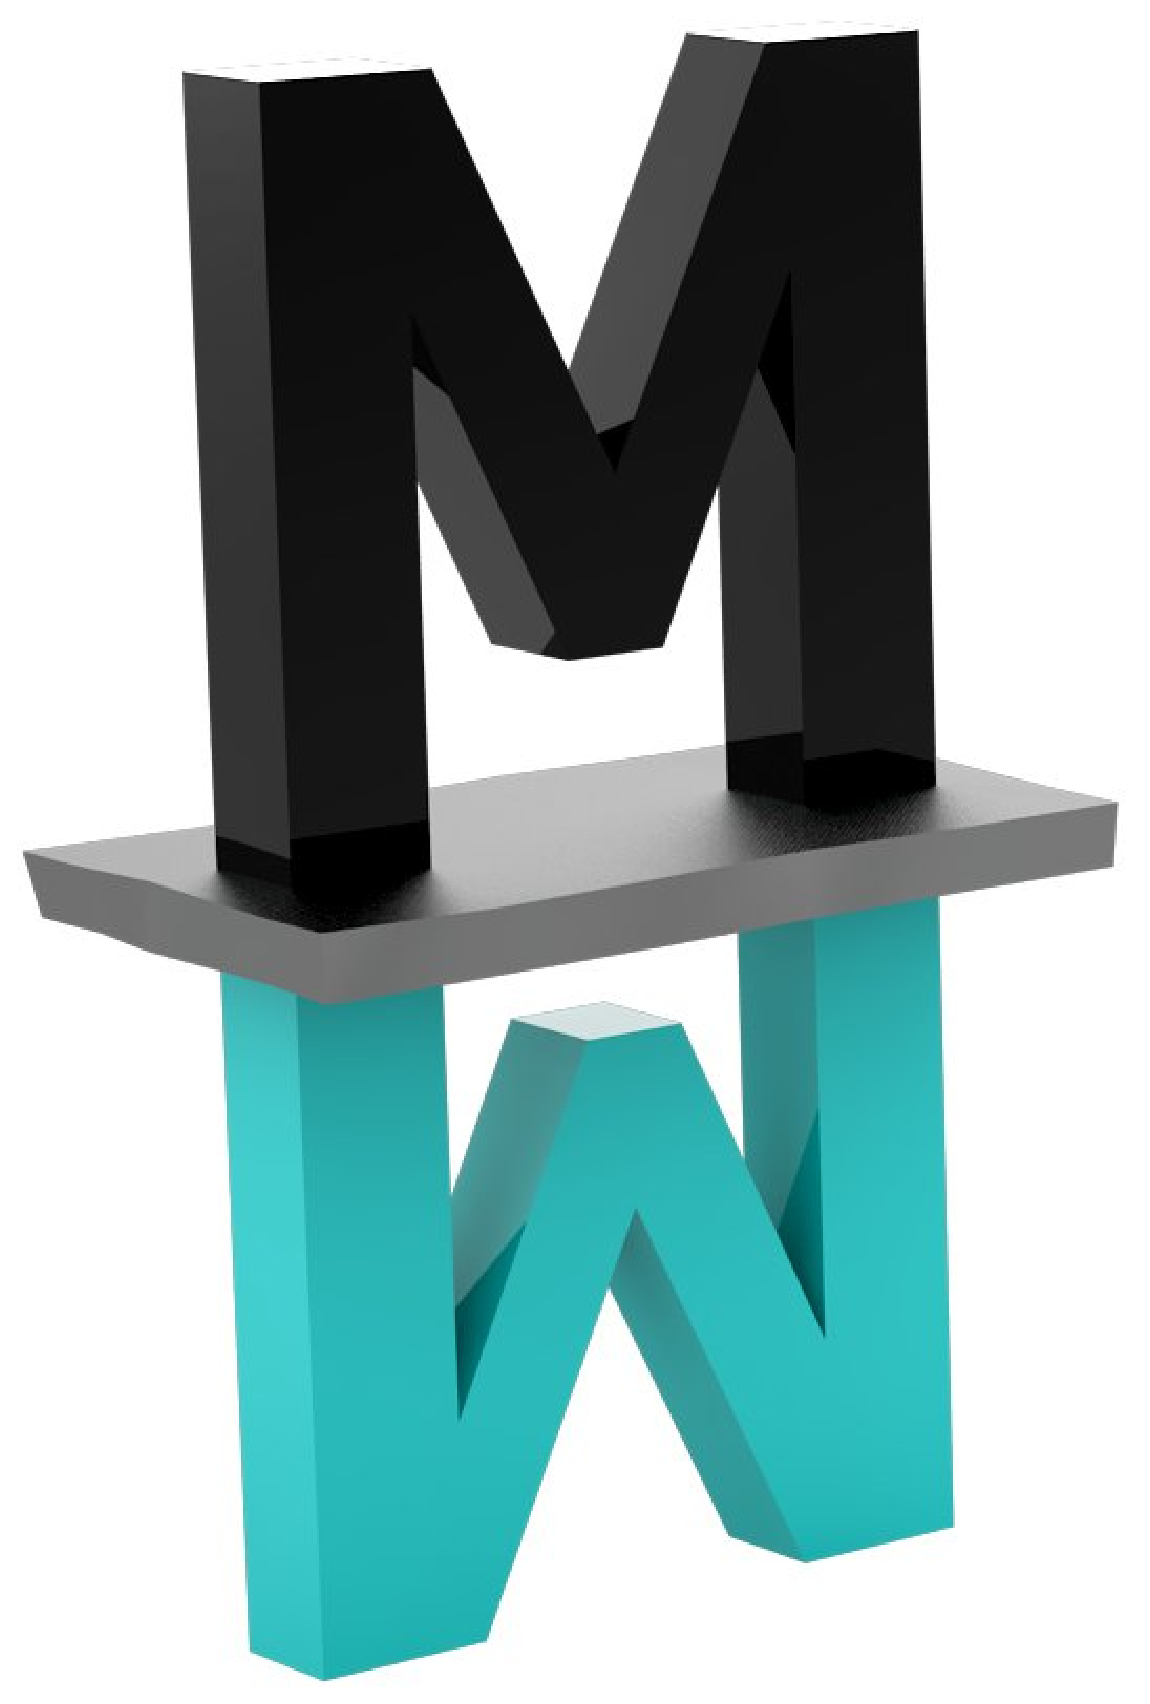
\includegraphics[height=80mm]{graphics/IMWlogo.eps}}                          % IMW logo
  \put(675,-20){
\includegraphics[height=18mm]{graphics/IMWname.eps}}                        % IMW name
  \put(683,5){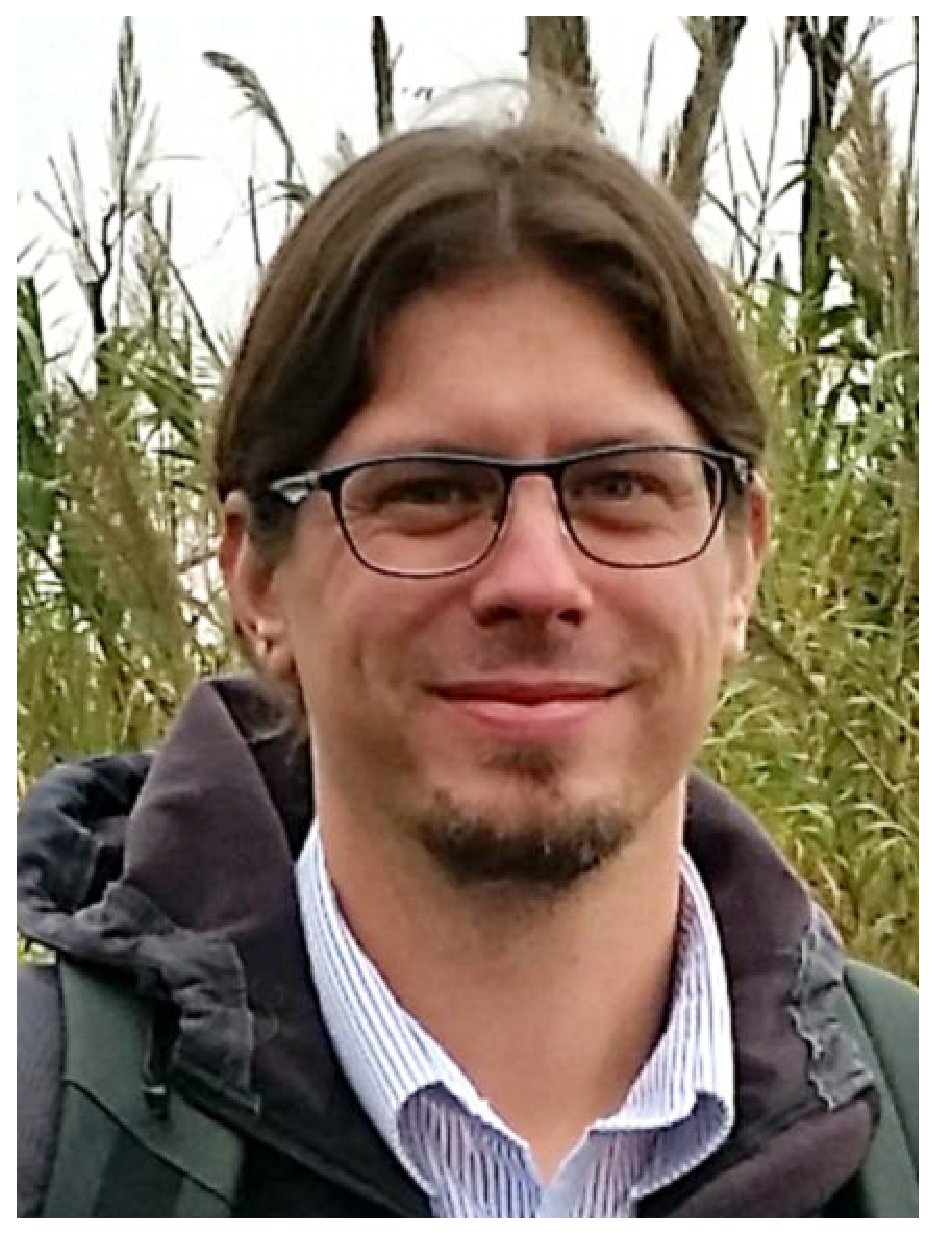
\includegraphics[height=70mm]{figs/david.eps}}                       % author's photo
  \put(683,10){\begin{pspicture}(0,0)                                              % frame around author's photos     
                \psframe[linewidth=2mm,linecolor=IMWgreen](0,-6mm)(54.5mm,66mm)
               \end{pspicture}}
  \put(79,62){\begin{pspicture}(0,0)                                               % poster title
                \psset{fillstyle=solid,fillcolor=white,linewidth=1.5pt,linecolor=IMWgreen,unit=1mm}
                \put(0,5){\pscharpath{\Huge\bfseries\scalebox{0.75}[1.]{Elasticity of interfaces: a multi-method approach}}}
              \end{pspicture}}1
  \put(75,30){\mbox{\parbox[b]{0.5\paperwidth}{\raggedright\Large\bfseries\color{white}        % authors
    \scalebox{0.75}[1.]{\underline{David Holec}}$^{1}$
    \scalebox{0.75}[1.]{, Nikola Koutná}$^{2,3}$
    \scalebox{0.75}[1.]{, Monika Všianská}$^{3}$
    \scalebox{0.75}[1.]{, Martin Friák}$^{3,4,5}$\scalebox{0.75}[1.]{,}
    \scalebox{0.75}[1.]{Paul H. Mayrhofer}$^{2}$
    \scalebox{0.75}[1.]{, and Mojmír Šob}$^{3,4,6}$\scalebox{0.75}[1.]
  }}}
  \put(80,22){\mbox{\parbox[t]{0.7\paperwidth}{\footnotesize\slshape\color{white}               % address
    $^1$Department of Physical Metallurgy and Materials Testing, Montanuniversit\"at Leoben, Austria\\    
    $^2$Institute of Materials Science and Technology, TU Wien, Vienna, Austria\\
    $^3$Institute of Physics of Materials, Academy of Sciences of the Czech Republic, Brno, Czech Republic\\
    $^4$Central European Institute of Technology, CEITEC MU, Brno, Czech Republic\\
    $^5$Department of Condensed Matter Physics, Faculty of Science, Masaryk University, Brno, Czech Republic\\
    $^6$Department of Chemistry, Faculty of Science, Masaryk University, Brno, Czech Republic\\
  }}}
  \put(420,-2){\mbox{\parbox[t]{0.2\paperwidth}{\color{white}\raggedleft\footnotesize
        \dhEmail{} david.holec@unileoben.ac.at\\
        \dhEmail{} nikola.koutna@tuwien.ac.at\\
        \dhEmail{} mafri@ipm.cz\\
  }}}         % email

%   \put(-100,-1085){
\includegraphics[width=1.12\paperwidth,height=4.4cm]{graphics/IMWbackground_full.eps}}   % footer background  
  \put(-50,-1085){\mbox{\color{white}\rule{27cm}{4.4cm}}}
  \put(-10,-1080){
\includegraphics[height=4cm]{graphics/logo_TUW.eps}} 
  \put(55,-1080){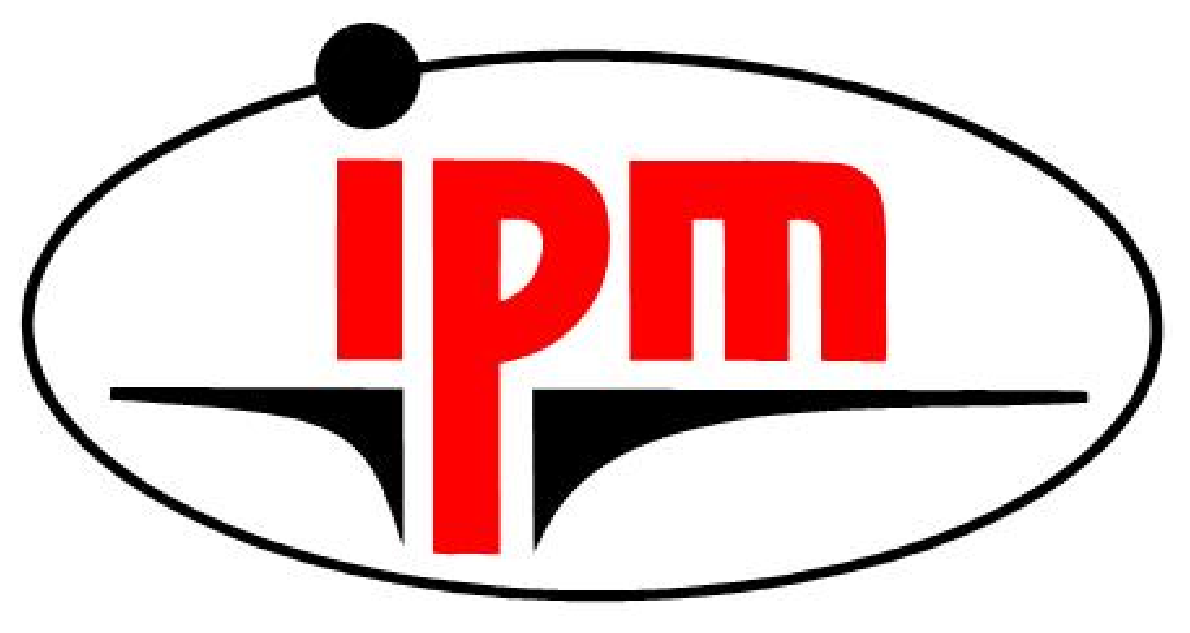
\includegraphics[height=4cm]{graphics/logo_IPM.eps}}   % collaborators
  \put(152,-1080){
\includegraphics[height=4cm]{graphics/logo_ceitec.eps}}
  \put(233,-1080){
\includegraphics[height=4cm]{graphics/logo_MU.eps}}
  \put(300,-1080){
\includegraphics[height=3.5cm]{graphics/logo_FWF.eps}}
  \put(420,-1080){
\includegraphics[height=4cm]{graphics/logo_VSC.eps}}
%   \put(450,-1080){\includegraphics[height=4cm]{graphics/logo_OeAW.eps}}
  \put(500,-1075){
\includegraphics[height=2.8cm]{graphics/logo_MetaCentrum.eps}}
%   \put(575,-1085){\mbox{\color{white}\rule{25cm}{4.4cm}}}
  \put(660,-1080){
\includegraphics[height=3.8cm]{graphics/logo_thermec}}
%   \put(230,-1067){\parbox{0.41\paperwidth}{\raggedright\footnotesize\color{white}\textbf{Acknowledgements: The computational results presented have been achieved [in part] using the Vienna Scientific Cluster (VSC).} }}      % acknowledgements
\end{picture}




\posterBox{20}(0,1){Introduction}{
  \begin{itemize}
    \item Intentionally and controllably designed \alert{non-trivial material architectures} can bring behaviour \alert{outperforming homogeneous bulk} materials.
    \item \alert{Superlatttices} represent perspective route for protective coatings. These, however, often require outstanding mechanical properties.
    \item For a knowledge-driven development of new systems, reliable and \alert{predictive modelling} is required.
    \item \alert{\textit{Ab initio}} methods are accurate but computationally expensive; \alert{continuum mechanics} treatment is affordable, but characterisation of interface and/or surface properties is required.
  \end{itemize}\medskip\centering
  \setlength{\fboxrule}{3pt}
  \fcolorbox{Red3}{white}{\parbox{10\TPHorizModule}{\vspace*{.5\TPHorizModule}\centering\alert{$\leadsto$} \Alert{Method of Grimsditch and Nizzoli} \cite{Grimsditch1985-af,Grimsditch1986-lh}\\\vspace*{.5\TPHorizModule}}}\bigskip
}

\posterBox{20}(21,1){The G\&N method}{
  \begin{minipage}{9\TPHorizModule}
    \alert{Linear-elasticity continuum model}-based on \alert{elasticity tensor}, \alert{molar ratio} and \alert{crystallographic orientation} of each individual phase.\medskip\\
%     
    \Alert{Limitations}:
    \begin{enumerate}
      \item {\alert{Neglects}} any heterogeneity introduced by the \alert{layer interface}.
      \item \alert{Neglects} the \alert{bi-layer period}.	
      \item The input $C_{ij}$s correspond to equilibrium \alert{lattice parameters} of each phases, which can differ from the in-plane lattice parameter of the superlattice.
    \end{enumerate}
    \vspace{-0.3\TPHorizModule}\mbox{}
  \end{minipage}\hfill
  \begin{minipage}{8.5\TPHorizModule}
    \alert{G\&N for 2 layers}: $\hat C_{ij}=\chi(\hat C_1, f_1, \hat C_2, f_2)$\medskip
    \begin{enumerate}
      \item $\hat P_i=\begin{pmatrix}
            1&0&0&0&0&0\\
            0&1&0&0&0&0\\
            C_{31}&C_{32}&C_{33}&C_{34}&C_{35}&C_{36}\\
            C_{41}&C_{42}&C_{43}&C_{44}&C_{45}&C_{46}\\
            C_{51}&C_{52}&C_{53}&C_{54}&C_{55}&C_{56}\\
            0&0&0&0&0&1
          \end{pmatrix}$
      \item $\hat M_i = \hat P_i^{-1}\hat P_1, i=1,2$
      \item $\hat M=\sum_{i=1}^2f_i\hat M_i$
      \item \alert{$C_{ij}(\text{bi-layer})=\big(\sum_{i=1}^2f_i\hat C_i\hat M_i\big)\hat M^{-1}$}
    \end{enumerate}\medskip
    Can be generalised for $N$ layers.
  \end{minipage}
}


\posterBox{14.5}(26.5,27){Conclusions}{
  \vspace*{-3mm}
  \begin{itemize}
    \item An explicit \alert{\textit{ab initio} elasticity} calculations of nitride \alert{superlattices and a grain boundary} in Ni$_3$Al intermetallic alloys.
    \item Continuum linear elasticity approach as formulated by \alert{Grimsditch and Nizzoli} was applied.\bigskip
    \item \Alert{CrN/AlN} superlattice yielded \Alert{excellent agreement} between explicit \textit{ab initio} elastic tensor and its approximation by the G\&N method.
    \item \Alert{Qualitative agreement} obtained also for majority of \Alert{MoN/TaN systems}.
    \item \Alert{The G\&N method fails} for the case of $\Sigma_5$ \Alert{GB} in Ni$_3$Al.\bigskip
    \item Reasons are:
      \begin{itemize}
        \item omission of \alert{interface-induced modifications of atomic/electronic structure},
        \item inability to reflect different \alert{bi-layer periods}.
      \end{itemize}
  \end{itemize}
}

\posterBox*{14.5}(26.5,38.25){References}{
  \let\oldbibliography\thebibliography
  \renewcommand{\thebibliography}[1]{\oldbibliography{#1}
  \setlength{\itemsep}{0pt}} 
  \bibliographystyle{aipnum4-1}
  \small\bibliography{refs}
}  

\posterBox*{14.5}(26.5,45.1){\scalebox{0.85}{Acknowledgements}}{
  \footnotesize
  asd
}
\end{document}
